\chapter[Introduction]{Introduction}
In today’s modern computing and rapidly evolving technological landscape, cloud-native technologies have become pivotal. These technologies extend beyond merely hosting applications in the cloud to fully leveraging the clouds inherent advantages, enabling the creation of secure, scalable and distributed applications. Cloud-native applications are designed to manage high concurrency, handle infrastructure failures gracefully and prioritize security from the outset. This architecture ensures applications are resilient and efficient, meeting the high demands of today's digital environment. \cite{r1}

Fundamentally, cloud-native applications share several key properties that distinguish them from traditional software. They operate globally, with data and services replicated in local data canters to minimize interaction latencies and ensure robust consistency models. The inherent scalability supports thousands of concurrent users, requiring meticulous synchronization and consistency in distributed systems. Cloud-native applications are designed to handle infrastructure flexibility, constant failure and robust design principles. They allow structural enhancement and continuous testing of new releases without interrupting the performance and integrated highly efficient security systems to guarantee a secure and continuous operations. These features make cloud-native architectures pivotal to modern computing environments. The layers of cloud-native application is shown in \autoref{fig:Cloud-Native Architecture}. \cite{r1}


\captionsetup{justification=centering}
\begin{figure}[h]
\centering

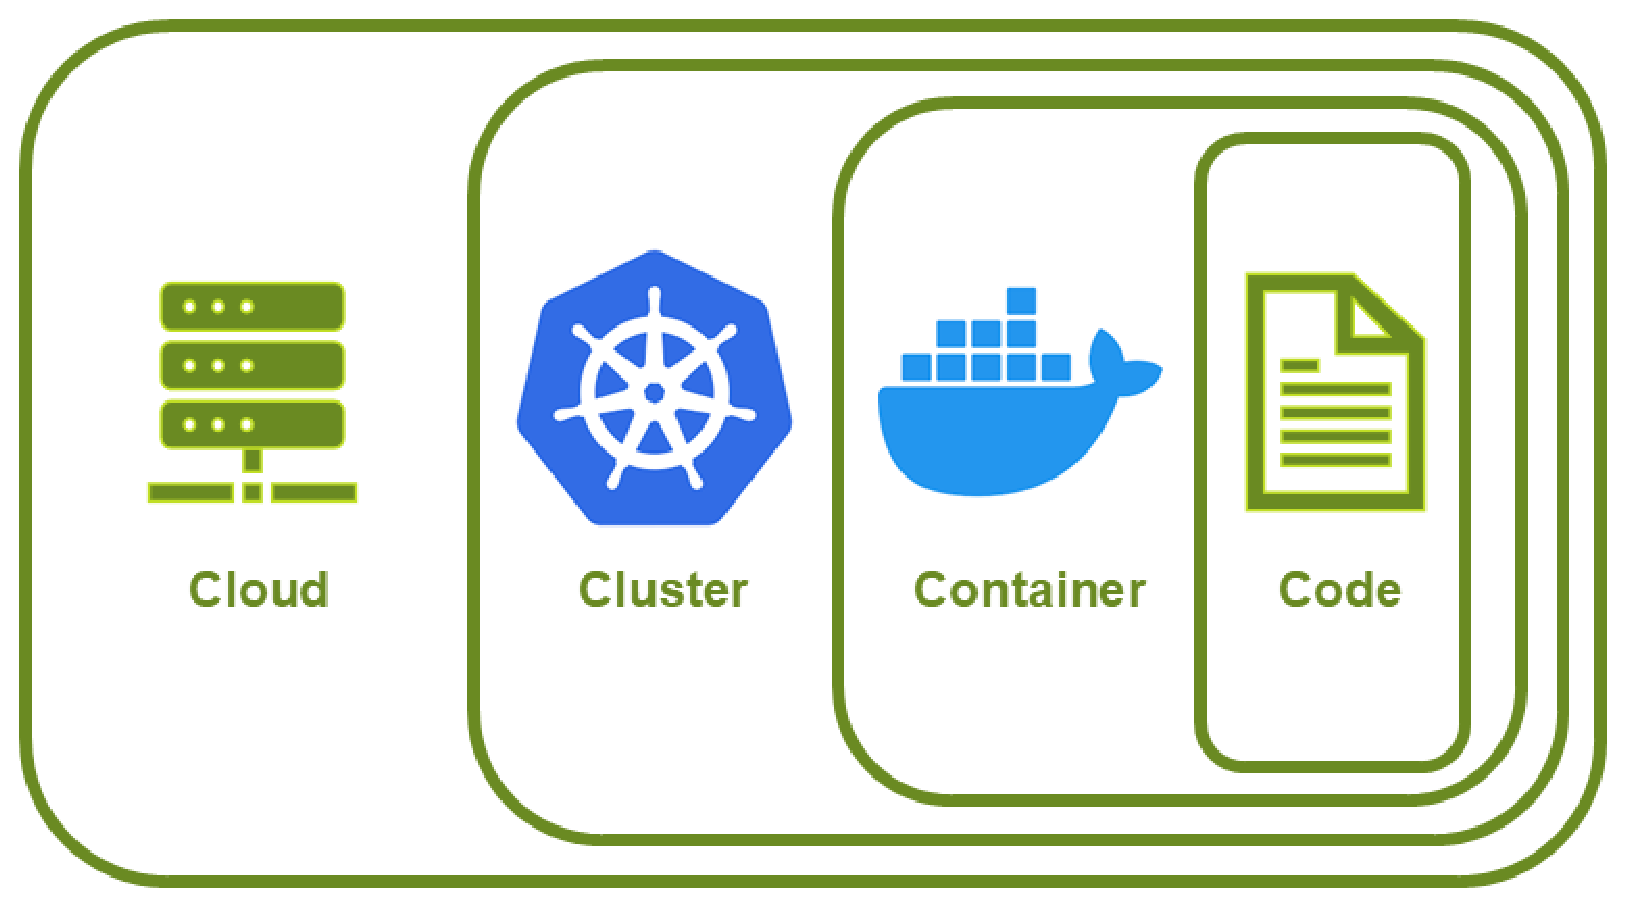
\includegraphics[width=0.8\textwidth]{Thesis/Figures/Slide2.pdf}
\caption{\label{fig:Cloud-Native Architecture}Cloud-Native Architecture \cite{r3}}
\end{figure}

\section{Background and Motivation}


This section describe the challenges of achieving secure, scalable and distributed computing and importance of the cloud-native architectures in modern computing.


\subsection{Importance of Cloud-Native Architectures in Modern Computing}

Cloud-native architectures represent a significant shift in modern computing, focusing on secure, scalable and distributed computation. These architectures are specifically designed for the cloud so application can be created and released quickly by small dedicated feature teams. Organizations who implement the cloud model are able to scale out and decouple from problematic hardware which in turn allows them more flexibility, fault tolerance and portability across different cloud environments. \cite{r2}

This further increases flexibility and resilience using containerization technology like docker and orchestration applications such as Kubernetes. Containers provide consistency across development, testing and production environments, while Kubernetes automates the deployment, scaling and operation of application containers. This infrastructure is adaptable to heavy loads and at the same Ɵme includes redundancy for a fault tolerant system. \cite{r4}



\subsection{Challenges in Security, Scalability and Distributed Computation}

In cloud computing, addressing the challenges of security, scalability and distributed computation is crucial for building robust and efficient cloud infrastructures. Each of these aspects presents unique difficulties that require careful consideration and strategic solutions to maintain the integrity, performance and reliability of cloud services. Security remains a paramount concern due to the inherent vulnerabilities introduced by multi-tenant environments, data transmission across networks and reliance on third-party services. The vulnerabilities range from cyber attacks, unauthorized access, and data breaches, thus data integrity, confidentiality and availability is paramount. Some of the risk can only be handled by implementing various security measures such as encryption, attribute-based access control \abk{ABAC}{Attribute-Based Access Control}, role-based access control \abk{RBAC} {Role-Based Access Control} and security audits. Scalability, is another critical aspect, which is the ability of a cloud system to handle varying loads efficiently. The elasticity of cloud-native architectures and flexible designs allow resources to be added or removed as needed based on usage. Scalability has several aspects, including performance, resources management and cost optimization. To achieve scalability in cloud-native architectures with autoscaling and load balancing and performance monitoring tools that guarantee an application’s capacity to scale without experiencing decline of quality of service. Distributed computation, which is fundamental to cloud computing, involves the coordination of multiple interconnected systems to perform complex tasks. The main challenges here include data synchronization, latency management, fault tolerance and ensuring coherent processing across distributed nodes. These challenges are compounded by the need for high availability and reliability in distributed systems. Implementing robust distributed algorithms, employing redundant systems and leveraging cutting-edge technologies such as container orchestration (e.g., Kubernetes) and microservices architecture can help address these issues effectively. Frameworks such as Ray streamline the development and deployment of distributed systems by simplifying distributed computation, providing a high-level interface for building scalable and resilient applications. \cite{r5}

Together, these challenges highlight the need for comprehensive strategies and advanced technologies to secure, scale and efficiently manage distributed cloud environments.

\subsection{Relevance of Research}

This research addresses the challenges discussed above by proposing a cloud-native architecture, aimed at enhancing the security, scalability and distributed computing. In this research, advanced tools are being employed such as Kubernetes for container orchestration \cite{r6}, Keycloak to implement authentication \cite{r7}, RBAC for authorization and access control and Ray for distributed computation \cite{r8}. The aim is to provide solutions to improve the efficiency, security and scalability of cloud-native architecture. 

\section{Objectives}

The objective of this research is to develop a synthesis of the foundational cloud-native architecture, which improves basic protection, expandability and parallel processing in Kubernetes environments. This involves three main research questions: 

\begin{itemize}

\item How can the principles of RBAC enhance security and improve administration in Kubernetes clusters by providing a foundation for access control and automating role provisioning?


\item How can Keycloak be integrated with ArgoCD to establish a secure single sign-on \abk{SSO}{Single Sign-On} mechanism using openID connect \abk{OIDC}{OpenID Connect} to streamline user authentication and enhance overall security?


\item How can Ray be used to enhance the scalability and efficiency of distributed machine learning workflows, including autoscaling of resources and graphics processing unit \abk{GPU}{Graphics Processing Unit} utilization and how does it compare with other available technologies?

\end{itemize}

\section{Scope}

This thesis focuses on the development of a cohesive cloud-native architecture that encompasses security, seamless authentication and optimized distributed computing within Kubernetes environments. The scope includes:

\begin{itemize}

\item Authentication optimization by integrating Keycloak with ArgoCD to enable a secure SSO mechanism with OIDC, which will streamline authentication processes and reinforce security measures within Kubernetes. \cite{r7}

\item Security enhancement through the deployment of RBAC in Kubernetes, covering the definition and application of Roles and ClusterRoles, as well as the automation of role management processes. \cite{r6}

\item Distributed Computation using Ray to improve the scalability and efficiency of machine learning tasks, including the distribution of computational workloads, dynamic resource management and GPU utilization within a Kubernetes environment. \cite{r8}
\end{itemize}

\clearpage

\section{Thesis Outline}

This thesis is structured into six chapters to systematically address the research objectives. Chapter 1 provides an introduction, starting with the background and motivation by highlighting the importance of cloud-native architectures in modern computing, the challenges in security, scalability and distributed computation and the relevance of this research. It outlines the primary objectives, briefly describes the scope of work covering key topics and gives an overview of structure of the thesis. Chapter 2 provide in-depth review of state of the art in cloud-native architectures, focusing on principles such as containerization, microservices and container orchestration. It explores best practices for scalability, security and distributed AI models. It also covers authentication and authorization tools and technologies for more effective and secure architectures. Chapter 3 then explain the methodology used to implement authentication, authorization and scalability in cloud-native architectures. It highlights the need for using SSO, access control and distributed computing methodologies. The chapter also also highlight how these methodologies are important when it comes to achieving secure, scalable and efficient cloud-native applications. Furthermore, Chapter 4 is dedicated to implementation which consists of sections such as Kubernetes, Keycloak, ArgoCD and Ray setups and it explains how authentication, authorization and scalable AI models were implemented. Chapter 5 compares Ray results with other distributed computing frameworks to highlight its strengths and weaknesses. Finally, Chapter 6 concludes the thesis by summarizing the research findings. It reviews the successful implementation of authentication, authorization and scalability mechanisms for the deployment of AI models. The chapter highlights how these components effectively address the key challenges of security, scalability and distributed resource management in a cloud-native architectures. It also presents suggestions for future work, that include the implementation of distributed computing frameworks for detailed performance analysis and the identification of the more scalable, compatible and efficient distributed computing framework.

